
In this section, we report the results of our work based on five complementary sets of analyses: 

\begin{itemize}
\item The geographical distribution of the listings.
\item The demographic composition of the hosts.
\item The services offered by the hosts.
\item The aesthetic presentation of the listings.
\item The pricing and ratings that hosts receive.
\end{itemize}


\subsection{Geographical distribution of \ab \ listings }

\begin{figure*}[!h]
\begin{center}
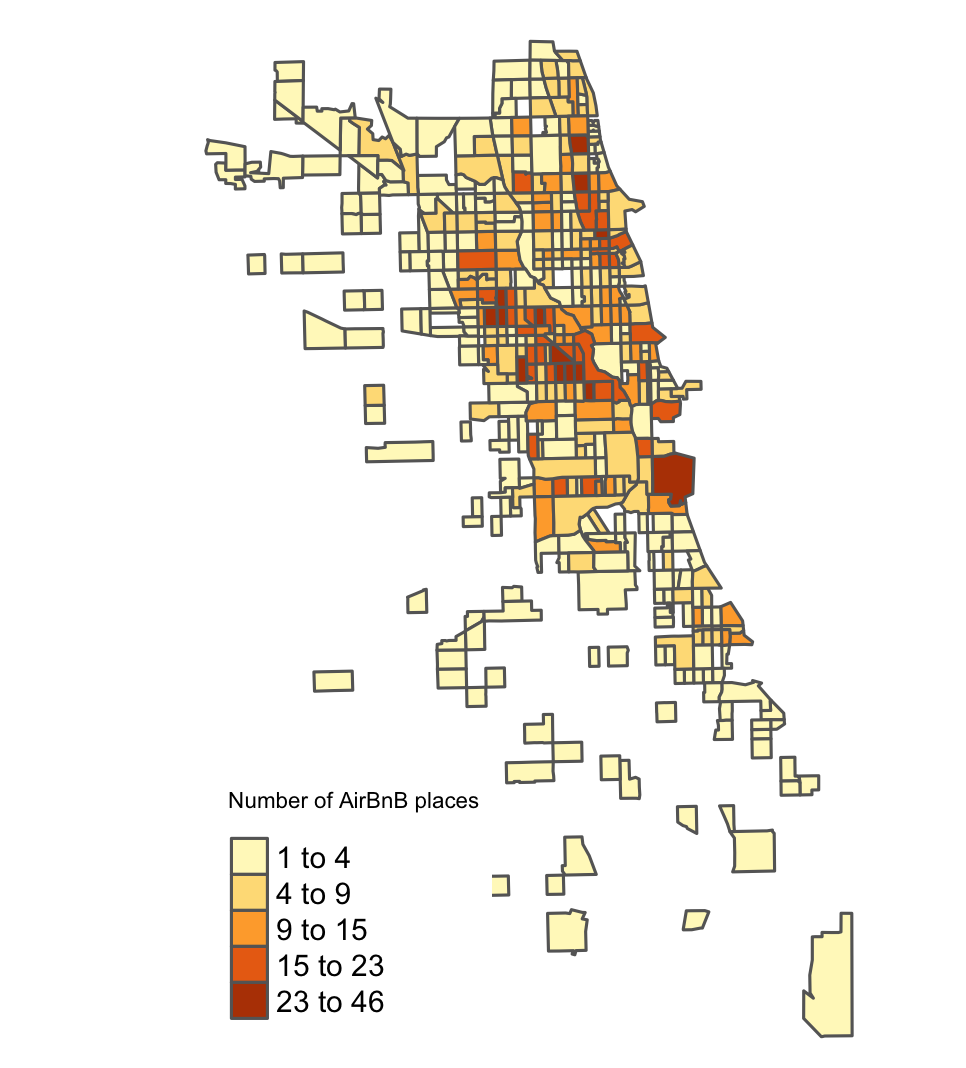
\includegraphics[scale=0.20]{pics/listings.png}
%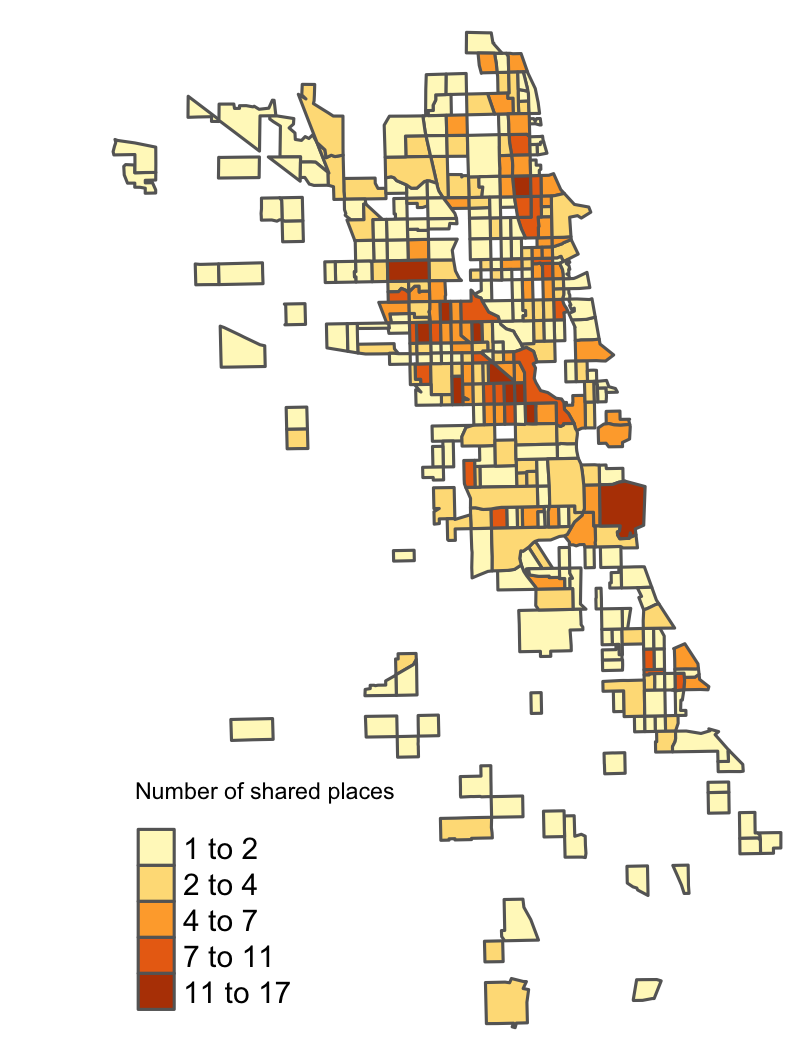
\includegraphics[scale=0.20]{pics/shared.png}
\caption{Geographical Distribution of AirBnB Listings (non-shared and shared).}
\label{fig:alllistings}
\end{center}
\end{figure*}

\begin{table}[htp] 
\begin{center}
\begin{tabular}{c|c|c}
& Median  Income & Household units \\
\hline
\hline
Number of Listings &  0.29 *** & 0.37 ***\\
%\hline
%Number of Shared &  0.20 *** & 0.25 ***\\
\hline
Number of Super-hosts &  0.24 ***& 0.18 ***\\
\hline
\end{tabular}
\end{center}
\caption{Pearson's correlation Coefficient and p-value. *** indicates p-value $\leqslant$ 0.001}
\label{tab:pre}
\end{table}%



%The examination of the geographical distribution of \ab \ listings in Figure~\ref{fig:alllistings}, presents the placements of all \ab \  listings as well as the subset of listings that were shared listings.
The examination of the geographical distribution of \ab \ listings in Figure~\ref{fig:alllistings}, presents the placements of all \ab \  listings.

As expected, most of listings are placed in the downtown area.
Furthermore, there are more listings in the richer northern suburbs of Chicago as opposed to the poorer and more racially diverse southern suburbs.

Pearson's correlation between the number of \ab \ listings and the census variables obtained from the American Community Survey (Table~\ref{tab:pre}), confirms that most properties are in richer and more dense areas, it also suggests that the super-host properties are placed in tracts with higher median household income.

%These results confirm previous findings in the literature, however this is at a high, aggregate level and does not provide insights into who the actual hosts are, their demographics and their offering on the \ab \ platform.


\subsection{Demographic analysis of the hosts}

Using the facial-recognition capabilities of Face++, we provide an overview of the demographic makeup of \ab \ hosts using an analysis of host profile pictures. Face++ predicts age, gender and ethnic background.

Face++ identified more than one person in 30\% of the host pictures.
These hosts and their listings were removed from our analysis, since  their identity could not be garanteed.

In the remaining 1700 hosts and their listings, Face++ reported, 47\% female 53\% male, 13\% Asian, 11\% African-American and 76\% White\footnote{Note that Face++ does not identify hispanic as a separate ethnic classification.} (Table~\ref{tab:age}).

\begin{table*}[h]
    \centering
    { \tablesize
    \begin{tabular}{l c c @{ } l}
    \multicolumn{1}{c}{\emph{Race}} &\emph{Percentage}     & \emph{Age Distribution}        &\emph{Female - Male}\\
    \hline
    Asian                         &  13\%     & \myhist{asianage}                 & 53\%-47\% \\
    African-American         &   11\%       & \myhist{blackage}       &  43\%-57\%\\
    White                            &   76\% & \myhist{whiteage}              &  48\%-52\%\\
    \hline
    \end{tabular}}
\caption{Demographic properties of \ab \ Chicago hosts based on the analysis of their profile picture.  }
\label{tab:age}
\end{table*}

%In order to understand the relation between these demographic variables (age, race and gender) and how the hosts use the \ab \ platform,

The cross-correlation matrix of demographic variables where the Pearson's correlation p-value is less than 0.01 (Figure~\ref{fig:correlation}), shows, as expected, that the number of reviews and reviews per month are highly positively correlated and also correlated with a super-host status. There was a weak positive correlation between super-host status and both age and membership duration (\emph{host\_duration}).

Interestingly, there is a positive correlation between age and white ethnicity, indicating that older hosts are more likely to be white, and a weaker negative correlation with gender, indicating that older hosts are more likely to be male.

%No other correlation between the type of the property (whether it is an entire place or shared) and other variables. 

 
\begin{figure}[h]
\begin{center}
%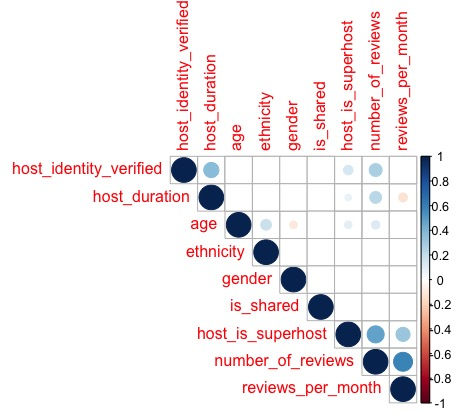
\includegraphics[width=\columnwidth]{pics/corplot.jpeg}
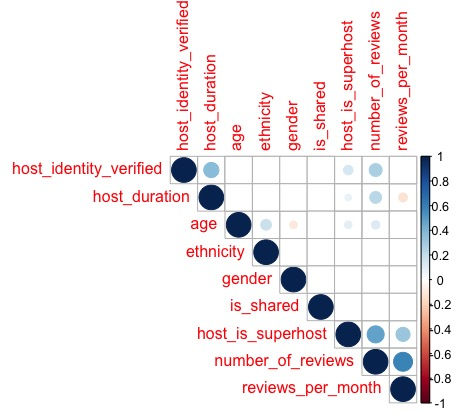
\includegraphics[scale=0.5]{pics/corplot.jpeg}
\caption{ Pearson cross-correlation matrix of the \ab \ platform features and the detected demographics where p-value significancy level is less than 0.01. Gender coded as female=1 and male=0 and ethnicity as white=1 and other=0. }
\label{fig:correlation}
\end{center}
\end{figure}


\subsection{Analysis of the properties offered }

Having examined the demographics of the \ab \ hosts for the dataset in hand, we now turn our focus to understanding what these hosts offer.   %Although the cross-correlation matrix did not support any correlation between the demographics variables and the type of the property (the entire property vs shared room)....<HERE> 

To this end, we calculate a residual metric which measures the discrepancy between the actual ethnicity ratio of the \ab \ hosts and the expected ratio based on the census population of these communities.

ratio of African-American/asian hosts in \ab \ 

We measure the actual ratio by dividing the number of African-American/Asian hosts by the total number of \ab \  hosts in each census tract.
We then calculate the residual by subtracting this measure from the ratio of  the census.
The higher the value of the ethnicity residual the bigger is the discrepancy between the ethnical background of the residents and the \ab \  hosts.
 
Figure~\ref{fig:gap} presents area cartograms  of the ethnicity gap for African-American and Asian population in the greater Chicago area.

In this figure, the tracts are colored according to the level of over- or under-representation, with a green color representing the tract with extreme under-representation of the African-American (or Asian) hosts compared to the residential population.

To put these discrepancy values into context,  we calculated two linear regression models with the dependent variable as the discrepancy value and census variables as independent variables (Table~\ref{tab:reg}).

As can be seen we observe a significant negative correlation with the median household income for the African-American discrepancy.

That is the poorer areas (those concentrated in southern part of Chicago) also exhibit higher under-representation in \ab.

This result indicates that those who could perhaps most benefit from the opportunities of micro-entrepreneurship are those who are not sufficiently represented in the system.  

\begin{figure*}[htbp]
\begin{center}
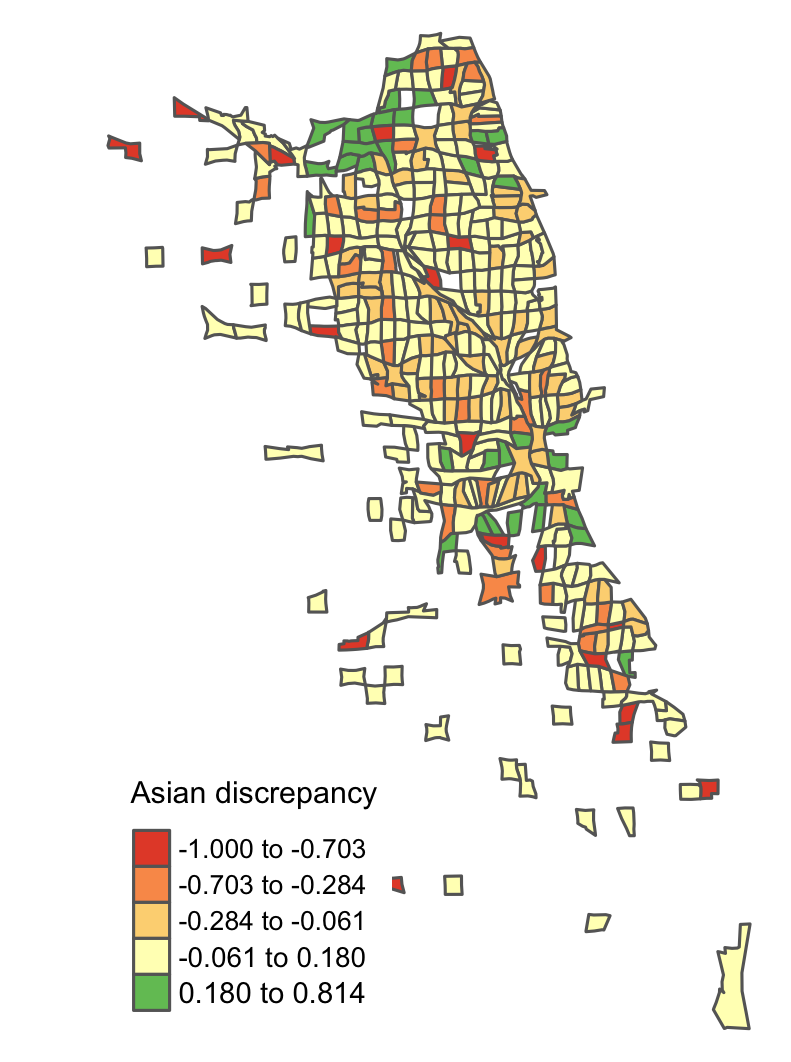
\includegraphics[scale=0.25]{pics/asian-gap.png}
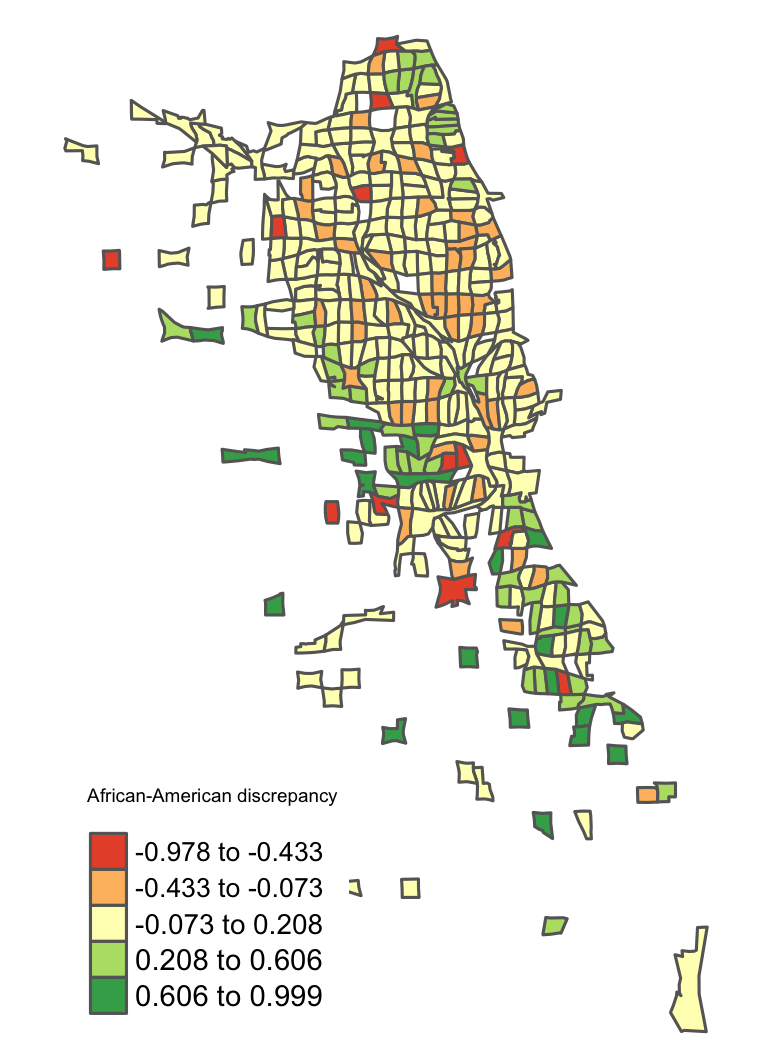
\includegraphics[scale=0.25]{pics/black-gap.png}

\caption{ An area cartograms based on the ethnicity gap where the green color (higher values) present areas in which there is the highest discrepancy between the ethnical background of the residents and the \ab \  hosts. }
\label{fig:gap}
\end{center}
\end{figure*}

 
   \begin{table}
        \centering

        \begin{tabular}{c|c c|c c}
%            \cline{2-5}
             & \multicolumn{2}{c}{African American } &  \multicolumn{2}{c}{Asian }\\
              \cline{2-5}
             & $\beta$ & p-value &  $\beta$ & p-value\\
           \hline
            \hline
              Median Income & -0.29 & *** & 0.00 &   \\
            No. Household & -0.07 & **  & 0.03 & . \\
            \hline
            \hline
            Adjusted R-squared    & \multicolumn{2}{c|}{ 0.224} &  \multicolumn{2}{c}{ 0.001}\\

        \end{tabular}
\caption{Regression analysis of the discrepancy value for African-American and asian communities in relation to the income and population data.  }
\label{tab:reg}
    \end{table}


\subsection{Aesthetic presentation of properties}
%here some stats on the scores. 
We now turn our attention to how the hosts present their properties on the \ab \ platform. Figure~\ref{fig:aes} presents the frequency distribution of the aesthetic scores of all the images. As it can be seen the distribution is skewed toward higher scores, demonstrating that most of the images in our dataset are both of good quality (local features), and well composed (global features). Indeed, we manually checked the images that had a very low aesthetic score (falling below the first interquartile range~-- IQR) and found that most of those images suffer from low local properties and in many cases are blurred. 

\begin{figure}[!h]
\begin{center}
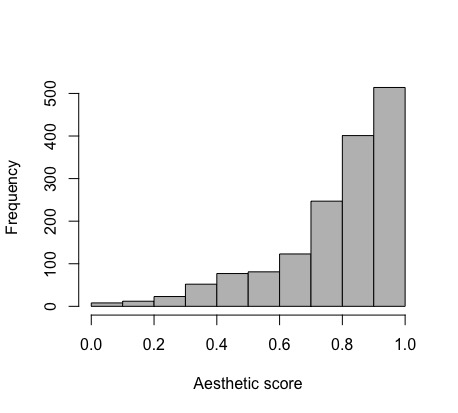
\includegraphics[scale=0.3]{pics/Hist-aes.jpeg}
\caption{The frequency distribution of the aesthetic scores of the main property photos. }
\label{fig:aes}
\end{center}
\end{figure}

Figure~\ref{fig:score} presents the choropleth map of the median aesthetic scores for each tract. We observe a weak positive correlation (r=0.14, p-value=0.005) between the median household income and the median aesthetic scores of the images, suggesting that hosts in the poorer neighborhoods do not present listings as well as others, perhaps due to socio-technical challenges. 

\begin{figure}[htbp]
\begin{center}
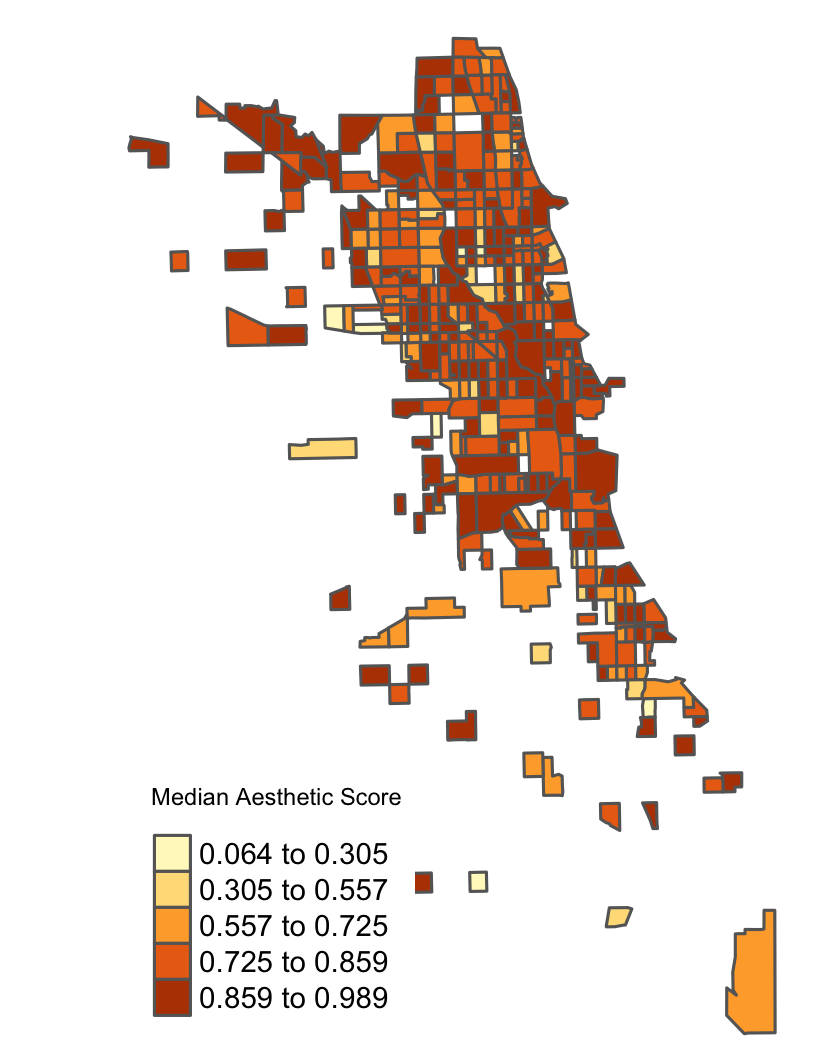
\includegraphics[scale=0.2]{pics/score.png}
\caption{The choropleth map of the median aesthetic scores. The lower shades present the areas with lower median aesthetic score. }
\label{fig:score}
\end{center}
\end{figure}


%We then conducted a  Welch Two Sample  t-test to compare the aesthetic scores between the hosts who had a property in the richest neighborhoods (where median income is higher than the third IQ) and those in the poorest neighborhoods  (where median income is less than the first IQ). The result of this analysis suggests that there is no significant difference between the two groups. That is being a host in a poorer neighborhood does not directly indicate poor quality of presentation on the platform. 


We then incorporate demographic of the hosts and conduct a series of  Welch Two Sample  t-tests  to compare the aesthetic scores between different i) female vs male ii) African-American vs white iii) asian vs white iv) super-hosts vs non super-hosts. We find no significant difference between the aesthetic scores of different genders. However, we find a significant difference in the aesthetic scores for the African-American (mean=0.75, sd=0.18) and White(mean=0.79, sd=0.18) hosts, with t(242)=-1.85 and p-value=0.03.  This gap widens even more (t(124)= - 2.31, p-value=0.01) when we compare the aesthetic scores for the African-American(mean=0.74, sd=0.18) and White (mean=0.8, sd=0.18) hosts in the neighborhoods where the median household income is in the first IQ (i.e., the poorest) and diminishes for the richer neighborhoods (with median income larger than the third IQ). Similar results were observed in comparing the aesthetic score of the Asian and White hosts.   Finally we find a significant difference (t(622)=2.09,p-value=0.01) between the aesthetic scores of super-hosts(mean=0.8, sd=0.17) compared to non super-hosts(mean=0.77, sd=0.19). We  do not observe any correlation between the aesthetic score of the images and the age of the host or the price of the property.  In summary, and complementing the prior section, it is primarily minorities from poorer neighborhoods that suffer from missteps in presenting their offerings.

%what is the relation between score and reviews 

Finally, we are interested in examining whether the aesthetic score actually has any impact on the host's success on the platform.
We use for this purpose the number of reviews per month as a proxy for demand and so an indicator of how successful a host is in renting out their property. We used reviews instead of ratings as an indicator of success because previous research has shown that  ratings are generally inflated and not very accurate~\cite{zervas2015first}. Furthermore Fradkin et al. have shown that more than  70\% of the times  people leave reviews after staying at a place~\cite{fradkin2015bias}.  As the popularity of a rental place is first and foremost dictated by its location, we calculate the median aesthetic scores and the median reviews per month for each census tract. We find a positive correlation of r=0.16 (p<0.001) between these two variables, indicating that the better the quality of the images, the higher the likelihood of the place being rented.   

A possible interpretation of these results is that hosts from a minority group and a lower socioeconomic background are those who require internal policies from \ab \ to assist them in presenting and offering their property on the platform. We discuss this implication in details in the next section.  

